% THIS IS AN EXAMPLE DOCUMENT FOR VLDB 2012
% based on ACM SIGPROC-SP.TEX VERSION 2.7
% Modified by  Gerald Weber <gerald@cs.auckland.ac.nz>
% Removed the requirement to include *bbl file in here. (AhmetSacan, Sep2012)
% Fixed the equation on page 3 to prevent line overflow. (AhmetSacan, Sep2012)

\documentclass{vldb}
\usepackage{graphicx}
\usepackage{balance}  % for  \balance command ON LAST PAGE  (only there!)
\usepackage{listings}


\begin{document}

% ****************** TITLE ****************************************

\title{IOT Traffic Simulation: {\ttlit Predictive Analysis}}
\subtitle{2016 Computer Science Senior Thesis}

% possible, but not really needed or used for PVLDB:
%\subtitle{[Extended Abstract]
%\titlenote{A full version of this paper is available as\textit{Author's Guide to Preparing ACM SIG Proceedings Using \LaTeX$2_\epsilon$\ and BibTeX} at \texttt{www.acm.org/eaddress.htm}}}

% ****************** AUTHORS **************************************

% You need the command \numberofauthors to handle the 'placement
% and alignment' of the authors beneath the title.
%
% For aesthetic reasons, we recommend 'three authors at a time'
% i.e. three 'name/affiliation blocks' be placed beneath the title.
%
% NOTE: You are NOT restricted in how many 'rows' of
% "name/affiliations" may appear. We just ask that you restrict
% the number of 'columns' to three.
%
% Because of the available 'opening page real-estate'
% we ask you to refrain from putting more than six authors
% (two rows with three columns) beneath the article title.
% More than six makes the first-page appear very cluttered indeed.
%
% Use the \alignauthor commands to handle the names
% and affiliations for an 'aesthetic maximum' of six authors.
% Add names, affiliations, addresses for
% the seventh etc. author(s) as the argument for the
% \additionalauthors command.
% These 'additional authors' will be output/set for you
% without further effort on your part as the last section in
% the body of your article BEFORE References or any Appendices.

\numberofauthors{5} %  in this sample file, there are a *total*
% of EIGHT authors. SIX appear on the 'first-page' (for formatting
% reasons) and the remaining two appear in the \additionalauthors section.

\author{
% You can go ahead and credit any number of authors here,
% e.g. one 'row of three' or two rows (consisting of one row of three
% and a second row of one, two or three).
%
% The command \alignauthor (no curly braces needed) should
% precede each author name, affiliation/snail-mail address and
% e-mail address. Additionally, tag each line of
% affiliation/address with \affaddr, and tag the
% e-mail address with \email.
%
% 1st. author
\alignauthor
Neeraj Asthana\\
       \affaddr{University of Illinois at Urbana-Champaign}\\
       \affaddr{Laboratory for Cosmological Data Mining}\\
       \affaddr{Urbana, Illinois}\\
       \email{neeasthana@gmail.com}
% 2nd. author
\alignauthor
Robert J. Brunner\titlenote{Senior Thesis Advisor}\\
       \affaddr{University of Illinois at Urbana-Champaign}\\
       \affaddr{Laboratory for Cosmological Data Mining}\\
       \affaddr{Urbana, Illinois}\\
       \email{bigdog@illinois.edu}
}
% There's nothing stopping you putting the seventh, eighth, etc.
% author on the opening page (as the 'third row') but we ask,
% for aesthetic reasons that you place these 'additional authors'
% in the \additional authors block, viz.
\additionalauthors{Additional authors: Anchal Agarwal ({\texttt{aagrawa4@illinois.edu}}), Vaishali Khandelwal ({\texttt{vaishali1216@gmail.com}}), and Rishabh Jain ({\texttt{rjain11@illinois.edu}})}
%\date{9 May 2016}
% Just remember to make sure that the TOTAL number of authors
% is the number that will appear on the first page PLUS the
% number that will appear in the \additionalauthors section.


\maketitle

\begin{abstract}
The goal and novelty of our project is to combine streamed GPS traffic estimation algorithms with road sensor data to accurately predict future traffic states and efficiently advise and direct drivers. Sensors are up and coming in cities and roadways soon \cite{Array of Things} and we hope to leverage these along with driver data to estimate conditions on road segments. This paper highlights the parameters for our model, the technical specifications, details on time decay model (along with our modifications), Spark Streaming code, and considerations for future work. Other papers by my collaborators \footnote{Anchal Agarwal, Vaishali Khandelwal, and Rishabh Jain who are cited below} will highlight the generation of weather and vehicle data as well as the technical system considerations and benchmarking. 
\end{abstract}




\section{Introduction}

\subsection{Problem Statement}
Traffic congestion and its associated effects such as air pollution and car accidents pose major concerns to people who are on the move. And this problem is only getting worse as congestion has increased dramatically during the past 20 years in U.S. cities. During this time, the number of hours lost each year by the average driver to congestion has increased by 300 percent. According to Newsweek, the average United States commuter spends an average of 42 hours stuck in traffic every year, resulting in an estimated 160 billion dollar loss from loss of productivity. Increasing the capacity of the roadways is expensive and, in some areas where land is scarce, is not an option. Currently, drivers are only informed by current and historical traffic conditions in their area and are not able to adequately equipped to understand future traffic states.

\subsection{Proposed Solution}
Many popular methods exist to predict traffic states by aggregating streamed GPS data (coordinates, velocities, and timestamps) of many vehicles. With the recent advances in sensor technology, infrastructure for estimating temperature, pressure, humidity, precipitation, etc. are readily available on roadways and can be used to determine driving conditions. The goal and novelty of our project is to combine streamed GPS traffic estimation algorithms with dynamic road sensor data to accurately predict future traffic states and efficiently advise and direct drivers. We will make use of the Time Decay model for aggregating stream GPS data presented in “Aggregating and Sampling Methods for Processing GPS Date Streams for Traffic State Estimation” \cite{Zhang:TimeDecay} and include methods to incorporate road sensor data. By incorporating both current traffic conditions and data from sensors on the road, we can understand how traffic may change on a single road segment in the near future (30 minutes, 1 hour, etc.). With an estimated future speed at each road segment, we can advise drivers with efficient and safe routes to their destinations. 

\begin{figure}
\centering
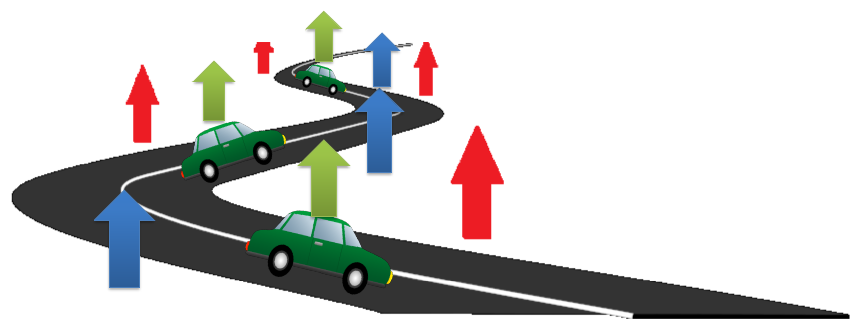
\includegraphics[width=3.5in,height=1.25in]{Road}
\caption{Cars and Sensors along a road segment generating data that can be processed by our system.}
\label{fig:road}
\end{figure}

\section{Data Sources}
There are two major data sources necessary for this project: streamed vehicle GPS data and road sensor data. These data sets are continually generated and streamed to our backend clusters. The data generation portions of the project were produced by my fellow project collaborators: Rishabh’s work focused on the generation of streamed GPS data while Vaishali’s work focused on generating road sensor data. Details on these methods can be found in other papers. 

\subsection{Streamed GPS Data}
Vehicles travelling along roadways continuously emit data to our backend server at a predefined interval (i.e. every second, every minute, etc.). Each emitted data packet from a vehicle will be of the form \textbf{(vehicle id, location, velocity, timestamp)} which can be abbreviated as ($id, v_i, l_i, t_i$). The vehicle id is a unique identifier for each vehicle. The location consists of a geodesic latitude and longitude coordinate. The velocity field consists of the vehicle’s current velocity which will be measured in meters per second. The timestamp references the time at which the location and velocity data was recorded in the form \textit{\%Y-\%m-\%d \%H:\%M:\%S}.

\subsection{Streamed Road Sensor Data}
Our model allows us to generalize to any number or type of sensor, however, for this paper we will only focus solely on a single type of sensor measuring road surface temperaturea. Sensors are placed along road segments at a predefined interval (i.e. every mile, every five miles, etc.) and our model assumes that these locations are known (mathcing road segment ids). Each sensor will periodically emit information to our backend server at a predefined interval (i.e. every second, every minute, etc.). Each road sensor data packet will be in the form: \textbf{(sensor id, temperature, timestamp)}. The sensor id is a unique identifier for each sensor. The temperature portion of the data packet defines a road surface temperature at the location of the sensor in Celsius degrees. The timestamp references the time at which the temperature was recorded in the form \textit{\%Y-\%m-\%d \%H:\%M:\%S}. In the future we will focus on extending our model to incorporate different types of sensors. Other potential sensor types include humidity, wind speed, water precipitation, etc. The data packet can be generalized as \textbf{(sensor id, observation, timestamp)} to accomodate these new sensor types. 

\section{Technical Specifications}
Our backend will be implemented on the NCSA ACX cloud computing cluster. We will be processing large amounts of data from vehicles and road sensors at small time intervals justifying the usage of large data clusters. The purpose of these systems is to efficiently stream and process data from vehicle and sensors sources to allow for future traffic state prediction. The focus of this paper will mostly be centered on the stream processing/cloud computing system, however, rough details of the other systems are also included. We will implement the Time Decay model mentioned later in the paper with the data streamed to cloud computing system from our message broker. A basic network diagram of the data flow is included in Figure 2 for reference. This section describes each of the systems and explains the basic actions taken at each step.

\subsection{Resources}

We have Kafka, Spark, and Cassandra systems setup on the ACX clusters. The specifications for each cluster are defined in Table 1 and details are provided in the next sections. 

\begin{table}
\centering
\caption{Specifications of resources setup on the NCSA ACX Cluster.}
\begin{tabular}{|c|c|l|l|} \hline
Cluster&Workers&Cores&RAM\\ \hline
KAFKA & 2 & 8 & 8 GB\\ \hline
CASSANDRA & 2 & 4 & 4 GB\\ \hline
SPARK & 6 & 24 & 17.2 GB \\ \hline
\end{tabular}
\end{table}

\subsubsection{Message Broker (\subsecit{Kafka})}
All vehicle and sensor data will be aggregated and ordered by a single message broker for efficient processing. Large amounts of real time data will continually be streaming into our backend and we use \textit{Apache Kafka} message broker which efficiently manages large amounts of messages. All the data captured at this step will be aggregated and ordered so that it can be sent to the data storage and stream processing units. The Kafka cluster contains two major queues, “traffic” and “weather”, known as topics. The “traffic” topic contains streamed vehicle data and each entry is of the form \textbf{(latitude, longitude, velocity, time, vehicle id)}. The “weather” topic contains streamed vehicle data and each entry is of the form \textbf{(segment id, time, measurement)}.

\subsubsection{Stream Processing (\subsecit{Spark})}
Spark is an open source computing cluster for large scale data processing and ideally suits our processing needs. The most recent data from the cars and the sensors will be sent to this unit to update the current road condition models using the time decay model. The newest data will be streamed into the system and be used (along with historical GPS data from the data store) to generate a new model describing the road conditions. Local variables will be persisted on all of the nodes in the Spark Cluster that store and update the parameters from the time decay model (details about the time decay model are provided in the following section). More details and specific code segments are provided about Spark Streaming are provided in the section below. There are considerations to also use or benchmark \textit{Apache Flink} or \textit{Apache Storm} in place of Spark as these may scale better to larger data streams however this must be tested further. 

\subsubsection{Database (\subsecit{Cassandra})}
All data will be stored in this unit to either be included in future models or displayed on the front end interface. The Cassandra table name is ``traffic'' with a schema of: traffic(id uuid, time\_stamp timestamp, latitude decimal, longitude decimal, PRIMARY KEY (id, time\_stamp)). This table will hold every traffic observation. We have not yet made a table to store road sensor data. \textit{HDFS}, \textit{HBase}, and \textit{MongoDB} have also been considered as replacements for this unit. 

\subsection{Data Pipeline}
Figure 3 details the general flow of the data between different clusters.  Data is generated by vehicles and road Sensors at a specified time interval (i.e. every second, mintute, etc.). This large stream of data is then aggregated and sorted by Kafka, placing the data into two separate streams (``traffic'' and ``weather''). The data is then sent to the Web Dashboard to display the current traffic conditions and it is also sent to the Spark Streaming instance to be processed into future speed predictions. The current conditions and predicted speeds are stored in a Cassandra database to be analyzed in depth at a later point. The future predcitions are also sent to the Web Dashboard which can then be displayed on consoles in vehicles. 


\begin{figure}
\centering
\includegraphics[width=3.25in,height=1.25in]{NetworkDiagram}
\caption{Network Diagram highlighting the major tasks occuring at each level.}
\label{fig:networkdiagram}
\end{figure}


\section{Time Decay Model}
Our model incorporates the Time Decay model suggested in “Aggregating and Sampling Methods for Processing GPS Date Streams for Traffic State Estimation” \cite{Zhang:TimeDecay} with road sensor data to estimate traffic states on specific road segments. We implement the aggregation based method mentioned in the paper as it requires minimal resources to implement and is efficient at estimating average speeds on road segments. We further adjusted the calculated average speed on each road segment based on data from road sensors from that same segment. 

The message broker (Kafka) sends vehicle packets of the form \textbf{(vehicle id, location, velocity, timestamp)} and each road sensor sends packets of the form \textbf{(sensor id, temperature, timestamp)}, which all will be ordered and aggregated by the message broker to form a stream and sent to the Spark Streaming system. 

\subsection{Velocity Estimation}
Previous models of estimating traffic states from GPS data streams focus on either historical data or a sliding window (SW) sampling methods. Historical methods attempt to aggregate previous speeds of vehicles on a particular road (each of which has an equal weight); however this method is not extremely accurate in the short term as GPS data streams are volatile and evolve rapidly based on different circumstances. The sliding-window sampling method conversely saves the most recent GPS data stream and uses only a select few point to estimate new traffic states. This also may not be completely accurate when estimating traffic states as it creates unstable traffic conditions that may not reflect the average behavior of a specific road. Therefore, we implement a time decay model which highly values new data records but also factors old data records. This method is also real time and easily updatable, allowing us to process data quickly and return current speeds on roadways. 

The key idea of the time decay model is to weight new records higher than old records on roadways. This is accomplished by weighting each record (\textit{i}) with a value \textit{w} using the following exponential decay function where \textit{i} represents the \textit{i}th GPS record, \textit{t} is the processing time of every observation, $t_i$ is the timestamp of the current record, and $\beta$ is some constant:

\begin{equation}w(i,t)=e^{\beta(t_i-t)}\end{equation}

where $\beta > 0$ and $t \geq t_i$.

Using this model, our system calculates time weights for each of the data records on a specific road segment and older records are weighted less than newer records. 

We also notice that high velocities are more useful than low velocities as low velocities can signal events that are not related to traffic flow such as parked vehicles or stopping at a red light. Therefore, we must weigh high velocity data as more important than low velocity data which is accomplished by assigning another speed weight to each record using a function \textit{g} that is positive, nondecreasing, and monotonic as follows where $v_i$ is the velocity of observation \textit{i}:

\begin{equation}w^v(i)=g(v_i)\end{equation}

Our model then assigns a full weight, $w^*(i,t)$, to a specific GPS data point by the following equation:

\begin{equation}w^*(i,t)=w(i,t) \cdot w^v(i) \end{equation}

For each predefined road segment, defined as \textit{r} (specifying a latitude and longitude radius), the estimated average velocity at time \textit{t} can be found using the following equation:

\begin{equation}\overline{V}(r)=\frac{\sum_{n=1}^{m} f(t_i - L) \cdot g(v_i) \cdot v_i}{\sum_{n=1}^{m} f(t_i - L) \cdot g(v_i)}\end{equation}


\subsection{Model Updates}

Equation 4 would be ideal for a batch processing system, however, it does not scale well to a fully streamed system that must constantly be updated to accomodate new observations. The model must be easily updated with newly streamed data points as well. In order to accomplish this, we will break $\overline{V}(r)$ into its numerator and denominator and define two new values \textit{X} and \textit{Y}:

\begin{equation}X = \sum_{n=1}^{m} f(t_i - L) \cdot g(v_i) \cdot v_i\end{equation}

\begin{equation}Y = \sum_{n=1}^{m} f(t_i - L) \cdot g(v_i)\end{equation}

The values \textit{X} and \textit{Y} will be persisted for each road segment and new observations can incrementally be added to these specific components. Then, whenever a velocity estimate ($\overline{V}(r)$) is needed, the values can be divided as $\overline{V}(r)=\frac{X}{Y}$.


\subsection{Incorporating Road Sensors}
The model described above is used only to get current estimates of speeds on roads and is not novel. Instead, our model incorporates road sensor data from road segments along with the estimated current velocity of those segments to project a future velocity on that same road segment (ex. In the next 30 mins, hour, etc.). Our current model only uses road surface temperatures with known parameters as a road sensor to predict a future speed, so these parameters are hard coded into our system. However, in the future when multiple sensors are used, we will use a machine learning algorithm (i.e. simple linear ridge regression) for each road segment to estimate future velocities using a variety of sensor data as inputs. 

\begin{figure}
\centering
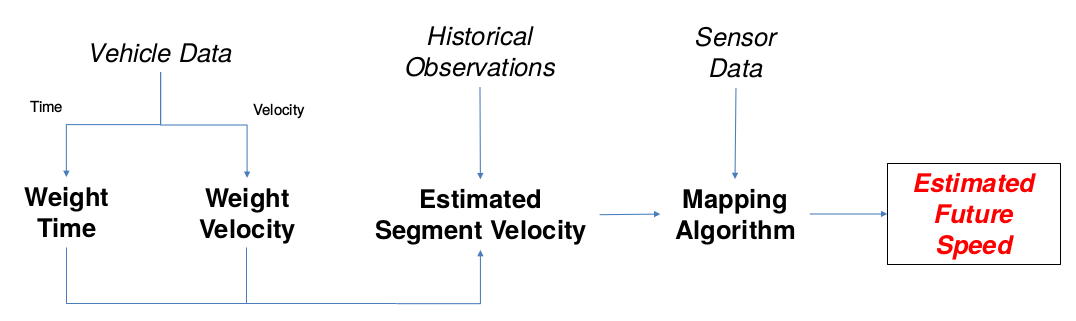
\includegraphics[width=3.25in,height=1.25in]{TimeDecay}
\caption{Describes how data flows through our modified Time Decay model to produce an estimated future speed.}
\label{fig:networkdiagram}
\end{figure}

\section {Dynamic Map Matching Algorithm}
Car data and road sensor data each have locations associated with each observation (latitude and longitudes) and must be matched to road segments in order to update specific model parameters. Therefore, we must translate a latitude and longitude observation to a specific road segment. 

\subsection{Code}
The current algorithm matches a road segment by find the closest road segment to the observation. The algorithm casts a radius of .25 kilometers from the location of the observation to accommodate for slight errors in GPS streamed locations. The code contains two key functions. The first function (distance) takes two latitude and longitude pairs as input and calculates the distance between them. The function is used to find the distance from an observation location to each road segment. 

\lstinputlisting[language=Python, firstline=22, lastline=37, frame=single]{all_code.py}

The second function (findSegment) attempts to find the closest segment to an observation’s location within a .25 km radius (for GPS error tolerance). The code cycles through all road segments and returns the closest one. If no segment is able to be matched, NONE is returned and the observation is skipped. 

\lstinputlisting[language=Python, firstline=40, lastline=52, frame=single]{all_code.py}

\subsection{Future Considerations}

In the future, we hope to be able to better distinguish between road segments by including a direction of travel field within each observation. In this way, we will be able to accurately match road segments if vehicles are at an intersection or close to another road. We will also be able to keep data for two way traffic (incoming and outgoing for a road segment). 


\section{Spark Streaming}
Apache Spark is an open source cluster computing engine for efficient and large-scale data processing (in real time). It also has simple integration libraries for Cassandra and Kafka, as well MLib (machine learning library). Spark Streaming allows for observations to continually added and updated as they are received. We used pyspark within an IPython Notebook to write and run our Spark commands. Applications are easily submitted to the cluster using a submit script using the \textit{spark-submit} command.


\subsection{Mechanics}
Spark holds its data in objects know as Resilient Distributed Datasets (RDDs) which in our case are created from vehicle and sensor data streamed from Kafka. Each RDD can then be transformed by operations (such as mapping, reducing, filtering, etc.) to generate the desired results. Spark Streaming creates a “DStream” for each Kafka queue which is essentially a series of related RDDs to represent a continuous stream of data. Each RDD in the DStream represents a specified time interval in the stream (every second, every minute, etc.), a single fetch from a Kafka queue. A sample visualization of data flow from cluster manager, driver, and the workers can be seen in Figure 4 \footnote{http://spark.apache.org/docs/latest/img/cluster-overview.png}. 

\begin{figure}
\centering
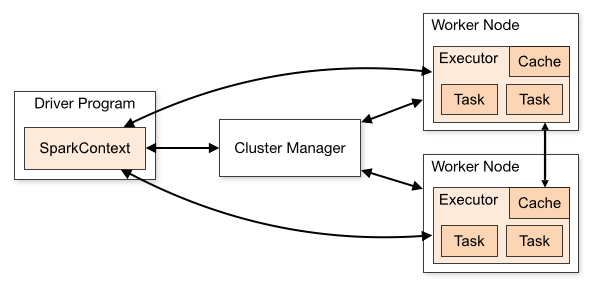
\includegraphics[width=3.25in,height=1.75in]{dstream}
\caption{Visualization of a Spark Streaming driver and workers data flow.}
\label{fig:dstream}
\end{figure}

Each Spark program contains a driver that handles organization and structure of each job submitted to the cluster. Other nodes and workers, then execute the transformational code in parallel and eventually accumulate a result. 

\subsection{State Preservation}
Each road segment is instantiated using the Segment class and all segments are held in the ``segments'' data structure, which is implemented as shared variables in Spark. This data structure will be updated and available on all Spark Nodes for efficient computing. 

\lstinputlisting[language=Python, firstline=16, lastline=16, frame=single]{all_code.py}

Each Segment object (instance of the Segment Class) has an \textit{id} and a \textit{location} (latitude and longitude). In addition, each segment object contains the parameters \textit{X} and \textit{Y} for that road segment (mentioned in section 4.2 and 6.3), the estimated velocity, and the number of observations the model is updated with. Lastly, the segment holds a landmark time (time of the first observation) and the time of the most recent observation, which are both used to weight observations in the time decay model. 

\lstinputlisting[language=Python, firstline=3, lastline=14, frame=single]{all_code.py}

\subsection{Model Update}

Vehicle and temperature data are streamed from Kafka at a specified time interval (i.e. every second) and each data stream is stored as a single Resilient Distributed Dataset (RDD) on a random worker node in the Spark cluster. Each observation in the stream is then matched to a road segment using the dynamic map matching algorithm (if possible from code mentioned in section 5.1). Map, Reduce, and Filter Python queries in batch and streaming mode are then used by PySpark to implement time decay traffic algorithm (mentioned in section 4.1). Each observation's velocity and time weights are calculated and then aggregated to update the \textit{X} and \textit{Y} values of the road segment. The matched road segment is then updated with the calculated values (speed, obs, time, \textit{X}, and \textit{Y}).

\lstinputlisting[language=Python, firstline=57, lastline=80, frame=single]{all_code.py}

These functions are then used as map and reduce operations by the Spark System. Each node operates on each observation in an RDD individually by associating and mapping a location using a dynamic matching algorithm (which represents a key for each observation). Each key is then aggregated using the time decay model update functions mentioned above in a reduce operation. The mapping and reducing is managed by a single master node (driver) that schedules and combines map-reduce tasks from different nodes.

\subsection{Spark-Kafka Integration}

Spark Streaming easily integrates with Kafka integration libraries and code is easily adapted to this change. The code that accomplishes this can be seen below. The basic step is to associate a Kafka Direct Stream with a Spark Streaming Context. The Kafka Direct Stream is inputed with a list of brokers (2 in this case) and a list of topics and a Spark Streaming Context. The Kafka Direct Stream can then be used with the same Time Decay code. All of this code is written to a file, ``timedecaykafka.py'', that will be submitted to the Spark compute cluster using the ``spark-submit'' command. The most important step is to include the jar in the submit script used to run the command on the cluster. The Streaming Context fetches data from the Kafka queues every 30 seconds however this time interval is easily adaptable as the application scales. 

\lstinputlisting[language=Python, firstline=83, lastline=110, frame=single]{all_code.py}

The following code is submitted to the command line to run the script above: \textit{!spark/spark-1.5.0-bin-hadoop2.6/bin/spark-submit} 

\textit{--master spark://10.0.3.70:7077 --packages org.apache.spark:spark-streaming-kafka\_2.10:1.5.0 timedecaykafka.py}.

\section{Future Work}

In the future we would like to incorporate many features into our models which were not possible to include during the spring semester. There are many optimizations and large scale features we hope to work on that could improve the system. 

\subsection{Dropped/Missing Data}
Not all data is properly delivered to our backend servers as receivers could lose service or turn off. We must adapt our model to successfully predict traffic conditions even when every piece of data is not completely available.

\subsection{Security}
How can we protect our network from hackers? The data and inferences provided by this model are extremely sensitive and proper authentication would be necessary to access this information. 

\subsection{Unidentified Vehicles}
Some vehicles are not equipped with GPS devices and we must adapt our models to incorporate these vehicles as well. These vehicles could skew different results from the Time Decay model (especially if there are large concentrations of unidentified vehicles) and we must remain agile amongst this uncertainty. 

\subsection{Variable Sensors}
Many types of sensors are available to monitor weather and traffic conditions. Currently, our model only uses road surface temperature sensors. However, we must incorporate other types of sensors into this model to try and see how different combinations of road conditions change vehicle behavior.

\subsection{Sliding Window}
After a certain period of time (based on chosen functions and constants), some observations may be weighted so minimally that they are insignicant in the model. So, thse insignificant and outdated observations inside the database and the Spark System can be deleted. A sample visualization of a Sliding Window can be seen in Figure 5 \footnote{http://spark.apache.org/docs/latest/img/streaming-dstream-window.png}. 

\begin{figure}
\centering
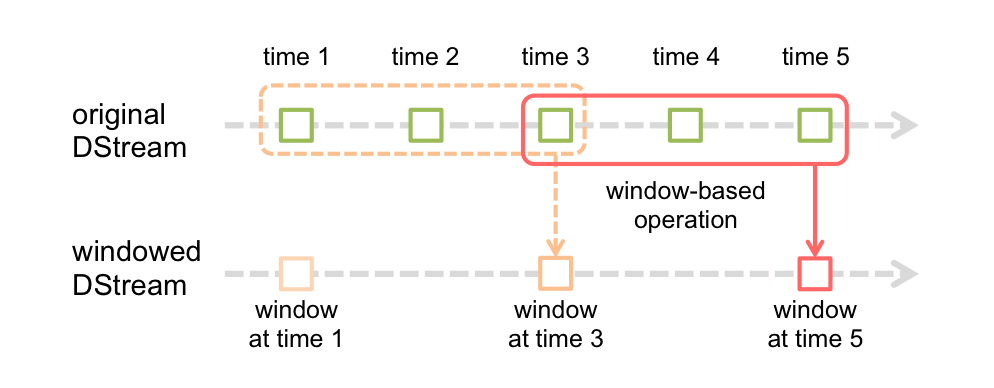
\includegraphics[width=3.25in,height=1.25in]{slidingwindow}
\caption{Visualization of a Spark Streaming Sliding Window at 5 different time intervals.}
\label{fig:dstream}
\end{figure}


\section{Acknowledgements}
We acknowledge support from the National Science Foundation Grant No. AST -1313415, the National Center for Supercomputing Applications, the University of Illinois and Microsoft Azure.


% ensure same length columns on last page (might need two sub-sequent latex runs)
\balance

%ACKNOWLEDGMENTS are optional


% The following two commands are all you need in the
% initial runs of your .tex file to
% produce the bibliography for the citations in your paper.
\bibliographystyle{abbrv}
\bibliography{vldb_sample}  % vldb_sample.bib is the name of the Bibliography in this case
% You must have a proper ".bib" file
%  and remember to run:
% latex bibtex latex latex
% to resolve all references

%APPENDIX is optional.
% ****************** APPENDIX **************************************
% Example of an appendix; typically would start on a new page
%pagebreak

Laboratory for Cosmological Data Mining

National Center for Computing Applications ACX Cluster

Apache Spark 1.5.0 Documentation → http://spark.apache.org/docs/latest/ 

Ipython Notebooks → http://ipython.readthedocs.org/en/stable/ 

Docker → https://docs.docker.com/ 

Spark-Ipython Notebook Integration → http://www.kuntalganguly.com/2015/06/configure-ipython-notebook-with-apache.html 

Cassandra → http://docs.datastax.com/en/cassandra/2.0/cassandra/gettingStartedCassandraIntro.html 

Time Decay Scholarly Paper Intelligent Transportation Systems, IEEE Transactions on, Issue Date: Dec. 2013, Written by: Jia-Dong Zhang; Jin Xu; Liao, S.S.

Kafka → http://kafka.apache.org/documentation.html 

https://arrayofthings.github.io/

\begin{appendix}

Our Ipython Notebook can be viewed at ``http:// 141.142.236.197:8888/ notebooks/Prediction/notebooks/Prediction.ipynb'' .

Setup for the Spark Cluster on the ACX Cluster can be found here: ``http:// 141.142.236.197:8888/edit/Infrastructure/SparkSetup.md''.

Setup for the Ipython Notebook Server on the ACX Cluster can be found here: ``http:// 141.142.236.197:8888/edit/Infrastructure/IpythonSetup.md''.

\end{appendix}



\end{document}
